%\usepackage{mathtools}
%\DeclarePairedDelimiter\ceil{\lceil}{\rceil}
%\DeclarePairedDelimiter\floor{\lfloor}{\rfloor}
%*********************第三章******************
\chapter{3D卷积神经网络在异构平台上的高性能实现}
\label{3DWinograd}
\section{引言}
卷积神经网络在图像分类、目标跟踪等很多2D输入的处理任务已经得到了成功的应用。卷积神经网络能够很好地提取特征,所以卷积网络常用于图像分类,比如Alexnet\ref{}、VGG\ref{} 、googlenet\ref{}、resinet\ref{}等卷积神经网络被用来对2D图像进行分类,达到了很好的分类效果。图\ref{}为经典的Alexnet网络,其主要包含大量的卷积层,其中的计算也主要集中在卷积层。

正因为2D卷积网络得到了广泛的应用,所以研究人员开始转向3D卷积神经网络的研究,在\ref{}已经为我们展现了一个名为ObjectNet3D用于3D物体识别的数据库,通过这个数据库的训练,可以达到识别3D的各种姿势的目的,类似于这样的3D数据库还有ShapeNet\ref{}。针对这些3D数据库的3D卷积网络也开始陆续被设计出来,比如Voxnet\ref{}就是一个用于解决3D物体识别的3D卷积神经网络,文章\ref{}提出用3D卷积神经网络解决人类动作识别的方法,此外, 3D卷积神经网络可以处理视频分类的应用\ref{}。

但对于3D卷积神经网络的应用来说,如果仍然采用2D卷积神经网络的方法来处理,就会存在计算量大,存储消耗大的问题。有些方法只能解决其中的一个问题,比如基于FFT变换的方法在某些情况下可以有效降低计算量,但是以消耗存储为代价的。有一种卷积计算的快速算法,称为WMFA(Winograd Minimal Filtering Algorithm),这种算法目前已经成功运用在2D卷积神经网络中,能够有效降低卷积中的计算量,并且不会增加额外的存储空间。因此,将2D WMFA应用到3D卷积神经网络中是非常值得研究的课题。本章内容主要是介绍3D WMFA算法在3D卷积网络上的应用,需要解决的问题包括,由2D WMFA算法的形式推倒出3D WMFA的形式;从理论上分析3D WMFA算法的复杂性,证明该算法在计算和存储开销上的优势;面向GPU异构平台,将3D WMFA算法高效地映射到GPU上。

本章内容安排如下:第二节介绍了关于卷积神经网络中加速的一些研究现状;第三节介绍快速卷积算法WMFA的3D形式,以及3D WMFA算法的复杂性分析并证明了3D WMFA在理论上可以减少卷积计算量;第四节将重点介绍3D WMFA算法的GPU实现,并且介绍了面向GPU的几种优化技术;第五节将对3D WMFA算法的性能进行评测,并与其它卷积方法的性能进行了对比;最后是对本章内容的总结,随着3D卷积网络应用的推广,对其进行加速变得尤为重要。

\section{相关研究}
对于卷积神经网络的加速,目前主要集中在对2D卷积神经网络的加速研究中,加速的方法主要包括网络结构的改进、算法的改进、深度学习框架中加速库的使用以及新的平台的使用。

Alexnet\ref{}是最早被提出的卷积神经网络,在图像分类应用中,与传统的机器学习分类方法\ref{}相比,分类精度得到大幅度提高,这也开启了对卷积神经网络研究的热潮。为了进一步提高效果,VGG\ref{}网络增加了卷积层的层数(最深多达19层卷积层),这样可以对待分类的图片提取更多的特征,提高分类的精度,虽然所有卷积核大小采用$3\times 3$的卷积核来控制计算量,但由于卷积层数多,计算量仍然很大。Network in Network(NIN)\ref{}是对卷积层的改进,卷积操作是一种线性变换,对特征为线性可分的输入分类效果会很好,而NIN就是解决输入为非线性可分的情况,NIN结构是在卷积层中间引入一个非线性变换操作。GoogleNet\ref{}的设计思路是通过增加网络的深度和宽度来提高分类的精度,但GoogleNet考虑到了计算量的问题,网络结构中引入了很多$1\times 1$的卷积核,该改进可以有效地防止计算量膨胀的问题。 squeezenet\ref{}网络结构在设计上也兼顾了计算量以及模型参数大小两方面,其主要优势就是在保证最后分类精度的情形下减少模型参数。

目前对于比较流行的深度学习框架,比如Caffe\ref{}、Tensorflow\ref{}、Theano\ref{}、Mxnet\ref{}等,它们都采用了专门优化的库实现其中的卷积计算。cblas是面向多核CPU的高效库,cuDNN\ref{}是面向Nvidia GPU的深度学习库。深度学习框架为深度学习开发者提供了一种非常简便的方式来开发深度学习应用,开发者只需要在配置文件中配置使用的平台,就能调用相应的库充分发挥这些底层平台的性能。

现有深度学习框架中调用的库中对卷积的实现大都是将卷积转化为矩阵乘的方法,矩阵分解的方法。。。。还有对卷积计算采用新的等价计算方法,比如FFT的方法\ref{}是将卷积转化为点乘,FFT方法针对卷积核比较大的卷积网络能够显著降低计算量,存在的唯一问题就是存储消耗过大。在卷积算法改进方面的研究还包括本章内容要介绍的应用到3D卷积网络的WMFA方法, Lavin\ref{}在GPU平台高效地实现了WMFA算法,取得了比cuDNN更好的性能。而在文章\ref{}中,作者面向的是FPGA平台,采用OpenCL实现了WMFA算法。无论是GPU平台还是FPGA平台,WMFA算法都表现了很好的并行性。

除了算法方面的改进,也有一些利用集群系统来提高卷积网络的性能。Adam等人开发的COTS HPC系统\ref{}是基于GPU服务器的集群系统,能够对大规模的神经网络进行训练。Google公司使用多年的分布式深度网络框架DistBelief\ref{}使用上千个CPU核心对几十亿的网络参数进行训练。Marthin等人\ref{}对训练的梯度下降法SGD\ref{}提出了一个高效的数据并行算法。H. Wang等人开发的MVAPICH2-GPU\ref{}针对集群中的InfiniBand连接,将CUDA集成在MPICH2中,从而解决了集群系统中的GPU间的通信问题,提高了MPI通信的效率。Mu Li等人\ref{}通过参数服务器的方法提高了在集群上训练的通信效率。

本章的工作主要是借鉴2D卷积网络中算法加速的相关研究,来加速3D卷积神经网络的计算过程。
\section{快速3D卷级算法}
本节将首先介绍3D卷积神经网络中的3D卷积计算的定义,然后通过对1D和2D WMFA算法的介绍,推导出WMFA的3D形式,并将3D WMFA 算法运用到3D卷积层的实现中,最后对3D WMFA算法的计算复杂行进行了分析。

\subsection{3D卷级神经网络定义}
对于2D卷积来说,每个卷积核有长和宽两个维度,卷积核在输入特征图的长和宽两个方向依次滑动进行卷积运算。假定2D卷积层的输入特征图规模为$N\times C\times H\times W$,卷积核规模为$C\times K\times R\times S$,则2D卷积按照其定义可以用公式\ref{eq:2dcnn}表示。
\begin{equation} \label{eq:2dcnn}
Y_{i,k,x,y} = \sum_{c=0}^{C-1}\sum_{r=0}^{R-1}\sum_{s=0}^{S-1}I_{i,c,x+r,y+s}F_{k,r,s,c}
\end{equation} 
3D卷积在2D卷积的基础上增加了深度维度的信息,因此卷积核在做卷积时也需要在深度所在维度进行卷积运算,公式\ref{eq:3dcnn}为3D卷积计算的公式。公式中 $Y_{i,k,x,y,z}$ 代表了第 $k$个通道的卷积计算结果, $I_{i,c,x+r,y+s,z+t}$ 为其中的一个输入特征图, $F_{k,r,s,t,c}$ 是其中的一个卷积核, 公式\ref{eq:3dcnn}是按照3D卷积的定义得到的计算公式,从公式中可以发现3D卷积计算的定义法需要消耗大量的计算,更为详细的复杂行分析将在\ref{Complexity}节中介绍。 

\begin{equation} \label{eq:3dcnn}
Y_{i,k,x,y,z} = \sum_{c=0}^{C-1}\sum_{r=0}^{R-1}\sum_{s=0}^{S-1}\sum_{t=0}^{T-1}I_{i,c,x+r,y+s,z+t}F_{k,r,s,t,c}
\end{equation} 

\subsection{3D WMFA 算法}
本小节将介绍一种快速的3D卷积实现算法,这里命名为3D WMFA算法,WMFA算法由\ref{}提出。WMFA最开始运用在1D和2D卷积计算中。下面将从1D和2D的WMFA形式推导出3D WMFA形式。

在1D的WMFA算法中,一次计算长度为$m$ 的块大小的结果,卷积核大小假定为$r$,则用$F(m,r)$来表示一次$m$个值的计算结果。按照1D卷积计算的定义,需要$2\times 3=6$次矩阵乘运算才能计算出$F(2,3)$,但如果采用1D WMFA算法,则卷积可以通过公式\ref{eq:1dwinograd}实现。
\begin{equation} \label{eq:1dwinograd}
F(2,3) = \begin{bmatrix}
i_0 & i_1 & i_2 \\
i_1 & i_2 & i_3 
\end{bmatrix}
\begin{bmatrix}
f_0 \\
f_1 \\
f_2
\end{bmatrix}
= \begin{bmatrix}
m_1 + m_2 + m_3 \\
m_2 - m_3 - m_4
\end{bmatrix}
\end{equation} 

其中,$m_1$、$m_2$、$m_3$以及$m_4$可以通过公式\ref{mequation}计算得到。

\begin{equation}
\label{mequation}
\begin{split}
m_1 = (i_0-i_2)f_0 	 \quad	m_2 = (i_1+i_2)\frac{f_0+f_1+f_2}{2} \\
m_4 = (i_1-i_3)f_2 	 \quad	m_3 = (i_2-i_1)\frac{f_0-f_1+f_2}{2}
\end{split}
\end{equation}

在1D WMFA中,乘操作的个数用$\mu(F(m,r))$表示,则$\mu(F(2,3))  = 2+3-1=4$,而在对输入的变换过程需要4次加法操作,卷积核的变换操作中需要3次加法操作。可以用公式\ref{matrices}这种矩阵形式来表示计算的过程。
\begin{equation} \label{matrices}
Y = A^T\begin{bmatrix}
(B^Ti)\odot{(Gf)}
\end{bmatrix}
\end{equation}

公式\ref{matrices}中的$A^T$、 $G$以及$B^T$为变换矩阵,对于$F(2,3)$来说,这些变换矩阵的具体值为式\ref{Mvalues}中所示。
\begin{equation} 
\label{Mvalues}
\begin{split}
B^T = \begin{bmatrix}
1 & 0 & -1 & 0 \\
0 & 1 & 1 & 0 \\
0 & -1 & 1 & 0 \\
0 & 1 & 0 & -1 
\end{bmatrix} \quad G = \begin{bmatrix}
1 & 0 & 0 \\
\frac{1}{2} & \frac{1}{2} & \frac{1}{2} \\
\frac{1}{2} & -\frac{1}{2} & \frac{1}{2} \\
0 & 0 & 1
\end{bmatrix} \quad A^T = \begin{bmatrix}
1 & 1 & 1 & 0 \\
0 & 1 &-1 & -1
\end{bmatrix} 
\end{split}
\end{equation}

在公式\ref{matrices},$i = {\begin{bmatrix}
i_0 & i_1 & i_2 & i_3
\end{bmatrix}}^T$  和 $f = {\begin{bmatrix}
f_0 & f_1 & f_2  
\end{bmatrix}}^T$分别代表了输入块以及卷积块。2D WMFA算法可以通过1D WMFA嵌套实现,正如\ref{}文章中描述的那样,2D WFMFA的形式如公式\ref{2DWMFA}所示。
\begin{equation}
\label{2DWMFA}
Y = A^T\begin{bmatrix}
\begin{bmatrix}
GfG^T
\end{bmatrix} \odot \begin{bmatrix}
B^TiB
\end{bmatrix}
\end{bmatrix}A
\end{equation}  
其中$f$是大小为$r \times r$的卷积核,$i$为大小为$(m+r-1) \times (m+r-1)$的图像块。同样地可以对2D WMFA的计算量进行简单的分析,计算$F(2\times 2,3\times 3)$,需要$4 \times 4 = 16$次乘操作,然而如果按照卷积的定义来计算卷积,需要$4 \times 9 =36$次乘法运算,可以看出2D WMFA算法在理论上可以减少乘法数量,减少的倍数为$\frac{36}{16}=2.25$,代价是在输入数据变换阶段增加32次加法操作,在卷积核变换过程增加28次浮点运算,以及在反变换中增加24次加法操作。对于一个卷积层来说,输入和输出的通道数往往较大,所以输入通道需要跟不同的卷积核做卷积,则变换之后的输入块就可以重复利用多次,重复利用的次数与输出通道数的数目一致。在卷积过程中,卷积核需要在输入通道的$x$和$y$两个方向滑动进行卷积运算,因此,每一个变换的卷积块也可以重复利用,重复使用的次数与输入通道中的子块个数相同。对于卷积的计算结果输出块来说,输出块需要在输入通道方向进行一个归约操作,反变换是在归约操作之后进行的,反变换的次数就由输出通道数决定了,因此在输入数据的变换、卷积核的变换以及输出结果的反变换阶段中的开销相对于点乘运算来说是相对比较低的。

由上所述,可以知道1D WMFA和2D WMFA的计算过程分4个阶段,第一阶段是对输入的Winograd变换过程,第二阶段是对卷积核的Winograd变换过程,第三阶段是对前两个阶段的变换结果进行点积运算过程,第四阶段是将第三阶段点积的结果进行一次反变换得到最后卷积的结果。下面基于1D和2D 的WMFA算法,先提出3D WMFA的3D Winograd变换算法,以计算$F(2\times 2 \times 2, 3 \times 3\times 3)$为例,1D Winograd变换只对输入在一个维度上变换,只需要左边乘以一个矩阵,而2D Winorad变换需要在两个维度上变换,因此对输入先左乘一个变换矩阵,然后再右乘一个矩阵进行第二个维度的变换。因此3D Winograd变换是在2D Winograd变换的基础上再进行一次变换。下面将对输入的变换、对卷积核的变换以及反变换统一成一般形式,算法\ref{winogradTransform}为3D Winograd变换算法的一般形式,算法中$T_m$表示变换矩阵,$T_m$可以是对输入进行变换的变换矩阵$B^T$,或者对卷积核进行变换的变换矩阵$G$或者是反变换的变换矩阵$A^T$。算法中输入$I_0$可以使卷积输入数据,也可以是卷积核或者是点积后归约的结果。3D Winograd变换算法其实就是做在三个维度做了三次变换,每一次变换其实就是一次1DWinograd变换。
\begin{algorithm}
\caption{3D winograd transformation}
\label{winogradTransform}
\begin{algorithmic}
\STATE Input:$I_0[in\_size][in\_size][in\_size]$ 
\STATE Temp array: $I_1[in\_size][out\_size][in\_size]$, $I_2[in\_size][out\_size][out\_size]$
\STATE Output: $I_3[out\_size][out\_size][out\_size]$
\FOR{$i=0$ to $in\_size$}
	\FOR{$j=0$ to $in\_size$}
		\STATE{$I_1[i][0:out\_size][j] =T_mI_0[i][0:in\_size][j]$}
	\ENDFOR
\ENDFOR

\FOR{$i=0$ to $in\_size$}
	\FOR{$j=0$ to $out\_size$}
		\STATE{$I_2[i][j][0:out\_size] =T_mI_1[i][j][0:in\_size]$}
	\ENDFOR
\ENDFOR

\FOR{$i=0$ to $out\_size$}
	\FOR{$j=0$ to $out\_size$}
		\STATE{$I_3[0:out\_size][i][j] =T_mI_2[0:in\_size][i][j]$}
	\ENDFOR
\ENDFOR
\end{algorithmic}
\end{algorithm}

2D WMFA算法中的点积计算与归约计算可以转换成矩阵乘运算,下面也将推导出3D WMFA算法中的点积计算与归约计算可以转换成矩阵乘运算。
\begin{equation}
\begin{split}
Y_{i,x,y,z,k} = \sum_{c=0}^{C-1}I_{i,c,x,y,z}\ast F_{k,c} = \sum_{c=0}^{C-1}A^T\begin{bmatrix}
U_{k,c}\odot V_{c,i,x,y,z}
\end{bmatrix}A \\
= A^T\begin{bmatrix}
\sum_{c=0}^{C-1}U_{k,c}\odot V_{c,i,x,y,z}
\end{bmatrix}A
\end{split}
\end{equation}

考虑上式在$C$通道上的归约操作:
\begin{equation}
\label{reductionEq}
M_{k,i,x,y,z} = \sum_{c=0}^{C-1}U_{k,c}\odot V_{c,i,x,y,z}
\end{equation} 

公式\ref{reductionEq}可以划分成一些小的矩阵乘,假定输出块的大小为$(\varepsilon,\eta,\nu)$,使用新的坐标索引表示$(i,\tilde{x},\tilde{y},\tilde{z})$ 代替$(i,x,y,z)$可以得到如下表示:
\begin{equation}
\label{mmply}
M_{k,i,\tilde{x},\tilde{y},\tilde{z}}^{\varepsilon,\eta,\nu} = \sum_{c=0}^{C-1}U_{k,c}^{(\varepsilon,\eta,\nu)}V_{c,i,\tilde{x},\tilde{y},\tilde{z}}^{(\varepsilon,\eta,\nu)}
\end{equation} 

公式\ref{mmply}代表的即为矩阵乘,并且该矩阵乘可以简化为公式\ref{mmsimplify}。
\begin{equation}
\label{mmsimplify}
M^{(\varepsilon,\eta,\nu)} = U^{(\varepsilon,\eta,\nu)}V^{(\varepsilon,\eta,\nu)}
\end{equation}

根据前面3D Winograd以及矩阵乘转化的推导,现在可以给出3D WMFA算法的全过程了,3D WMFA算法包含4个阶段,首先是针对输入特征图的Winograd变换,其次是对卷积核的Winograd变换,然后是两个变换结果转化成的矩阵乘运算,最后是对矩阵乘的结果进行反变换得到最终的结果。算法\ref{3DWinograd}为该过程的详细介绍。
\begin{algorithm}
\caption{3D Convolutional layer implemented with WMFA $F$($m \times m \times m$, $r \times r \times r$)}
 \label{3DWinograd}
\begin{algorithmic} 
%\STATE P=$N\ceil{\frac{M}{m}}\ceil{\frac{P}{m}}\ceil{\frac{Q}{m}}$ is the number of image tiles.
\STATE P=$N{\frac{M}{m}}{\frac{P}{m}}{\frac{Q}{m}}$ is the number of image tiles.
\STATE $\alpha = m+r-1$ is the input tile size.
\STATE Neighbouring tiles overlap by $r-1$.
\STATE $d_{c,b}\in \!R^{\alpha\times\alpha\times\alpha}$ is input tile $b$ in channel $c$.
\STATE $g_{k,c}\in \!R^{r\times r \times r}$ is filter $k$ in channel $c$.
\STATE $Y_{k,b}\in \!R^{m\times m \times m}$ is output tile $b$ in filter $k$.
\FOR{$k=0$ to $K$}
  \FOR{$c=0$ to C} 
    \STATE{$u = T_k(g_{k,c}) \in \!R^{\alpha \times \alpha \times \alpha}$}
    \STATE{Scatter $u$ to matrices $U$: $U_{k,c}^{(i,j,k)} = u_{i,j,k}$} 
  \ENDFOR
\ENDFOR

\FOR{$b=0$ to $P$}
  \FOR{$c=0$ to C} 
    \STATE{$v = T_d(d_{c,b}) \in \!R^{\alpha \times \alpha \times \alpha}$}
    \STATE{Scatter $v$ to matrices $V$: $V_{c,b}^{(i,j,k)} = v_{i,j,k}$} 
  \ENDFOR
\ENDFOR

\FOR{$i=0$ to $\alpha$}
  \FOR{$j=0$ to $\alpha$} 
    \FOR{$k=0$ to $\alpha$}
      \STATE{$M^{(i,j,k)} = U^{(i,j,k)}V^{(i,j,k)}$}
    \ENDFOR 
  \ENDFOR
\ENDFOR

\FOR{$k=0$ to $K$}
  \FOR{$b=0$ to $P$} 
    \STATE{Gather $m$ from matrices $M$: $m_{i,j,k} = M_{k,b}$}
    \STATE{$Y_{k,b} = T_m(m)$}
  \ENDFOR
\ENDFOR
\end{algorithmic}
\end{algorithm}


\subsection{3D WMFA 算法的复杂性分析}
\label{Complexity}
这一节将对3D WMFA算法的计算复杂行进行分析。首先还是假设输入特征图的规模为$N \times C \times D \times H \times W$,卷积核规模为$K \times C \times r \times r \times r$,输出特征图的大小规模为$N \times K \times H \times W \times D$。 则3D WMFA算法中转化成的矩阵乘中的乘加操作总数可以通过公式\ref{mmnumber}表示。
\begin{equation}
\label{mmnumber}
%L_1 = 2N\ceil{\frac{M}{m}}\ceil{\frac{P}{m}}\ceil{\frac{Q}{m}}CK(m+r-1)^3
L_1 = 2N{\frac{H}{m}}{\frac{W}{m}}{\frac{D}{m}}CK(m+r-1)^3
\end{equation}

如果采用直接卷积的方法,需要总的浮点运算次数可以通过公式\ref{directNum}表示。
\begin{equation}
\label{directNum}
L_2 = 2NHWDCKr^3
\end{equation}

将公式\ref{directNum}与公式\ref{mmnumber}两边相除,可以得到它们的比值的表达式:
\begin{equation}
\frac{L_2}{L_1} = \frac{m^3*r^3}{(m+r-1)^3}
\end{equation}

为了看出3D WMFA算法的优势,假定$m=2$ and $r=3$,计算复杂性可以降低$\frac{L_2}{L_1}$ = $\frac{2*2*2*3*3*3}{4*4*4}$=$\frac{216}{64}=3.375$。然而3D WMFA算法在对输入、输出以及卷积核的变换中会增加一些加法的额外开销。也可以从理论上对这些额外的开销进行量化。假定对最小的输入块的变换开销为$\beta$,对卷积核块的变换开销为$\gamma$,对输出块的变换开销为$\delta$,这三个变换过程总的算术复杂性记为$T(I)$,$T(F)$,$T(O)$,则可以用公式\ref{transformComp}来表达。
\begin{equation}
\label{transformComp}
	\begin{split}
	%\frac{L_2}{L_1} = \frac{m^3*r^3}{(m+r-1)^3}
	T(I) = \frac{\beta}{m^3}NHWDC \\
	T(F) = \gamma CK \\
	T(O) = \frac{\delta}{m^3}NHWDK  
	\end{split}
\end{equation}

下面可以计算出各个变换阶段的计算复杂性占点乘阶段开销的比例,如公式\ref{transformMR}所示。从式中可以看出,对输入、输出以及卷积核的变换开销占点乘的比例是很低的。
\begin{equation}
\label{transformMR}
	\begin{split}
	%\frac{L_2}{L_1} = \frac{m^3*r^3}{(m+r-1)^3}
	T(I)/L_1 =\frac{\beta}{2K(m+r-1)^3}   \\
	T(F)/L_1 = \frac{\gamma m^3}{2NHWD(m+r-1)^3} \\
	T(O) /L_1= \frac{\delta}{C(m+r-1)^3} 
	\end{split}
\end{equation}

\section{3D WMFA 算法的实现与优化}
本节将对3D WMFA的具体实现进行介绍,面向的计算平台是GPU异构平台。在将3D WMFA算法映射到GPU中,需要针对GPU的体系结构特点进行一些相应的优化,从而提高3D WMFA算法在GPU上的性能。

\subsection{3D WMFA 算法的实现}
\label{baselineIm}
根据算法\ref{3DWinograd}的计算特性,该算法具有很好的并行性,因此采用GPU平台可以高效地实现算法\ref{3DWinograd}的各个计算过程。下面介绍3D WMFA算法的基本实现,基本实现的计算流图如图\ref{computeflow}所示,从图中可以看出3D WMFA算法的基本实现中包含的计算过程,首先是对输入特征图和卷积核的3D Winograd变换,变换之后的两个结果并没有直接进行矩阵乘运算,这里需要对变换之后的结果进行一次重排,数据按照矩阵乘所需要的存储格式重新组织,然后对重排之后的结果进行矩阵乘运算。矩阵乘在GPU上已经有可调用的高性能库,这里直接调用cublas实现矩阵乘。矩阵运算结束后也需要对结果进行一下重排才能进行反变换得到最后的结果。
\begin{figure*}[tbh]%\small
\centering
\resizebox{0.8\textwidth}{!}{
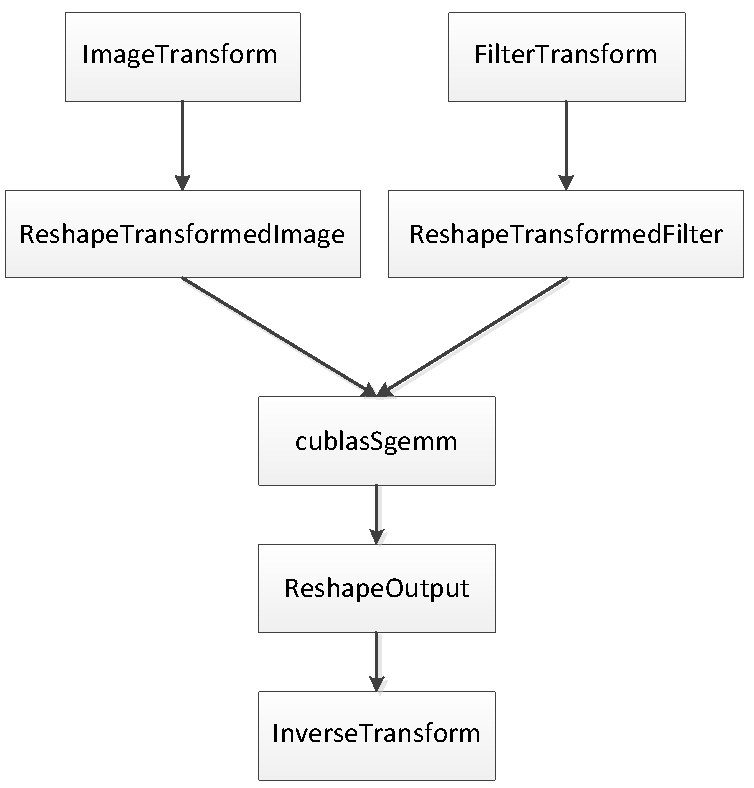
\includegraphics{figs/computeFlow.pdf}
}
\caption{The computing flow of 3D WMFA}
\label{computeflow}
\end{figure*}

在图\ref{computeflow}中,除了矩阵乘部分可以调用cublas库实现外,其它六个计算部分需要自己实现相应的CUDA代码。对于其中的三个变换来说,不管是输入图片还是卷积核或者输出,它们被划分成大量的小块,这些小块的变换都是相互独立的,所以可以并行执行,这个特点非常适合利用GPU进行加速实现。

以$imageTransform$ 这个kernel为例,它将实现对输入图片的3D Winograd变换,输入图片的规模为$N \times C \times D \times H \times W$,其中$N$为$batch$大小,$C$为输入通道数,$D \times H \times W$为单通道的规模。正如算法\ref{3DWinograd}中所说,每个通道中的图片小块个数为$P$,因此总的图片小块个数为$P \times C$,所有的图片小块的3D Winograd变换都是相互独立的,因此,这些小块的3D Winograd变换可以并行的执行。对于GPU上的$baseline$实现来说,输入图片的存储是按照$NCDHW$的顺序存储的,GPU上并发执行的线程是按照每个线程块中设置32个线程,这32个线程在一个维度上顺序排列,线程块的个数设置成三维的,具体值为$(\frac{N}{32},\frac{D}{m},\frac{H}{m},\frac{W}{m},C)$,因此总的线程个数与输入图片划分成的小块个数是一致的,每个线程完成一个小块的3D Winograd变换。由于线程块个数庞大,可以很好地发挥GPU的性能。

而对于卷积核的变换,在GPU中通过$fiterTransform$ kernel来实现,共有$K \times C$个卷积核需要变换,每个线程块中仍设置成32个线程,线程块的配置为$(\frac{K}{32},C,1)$,每个卷积核的变换也是可以并行地执行。

GPU的baseline实现中,在调用cuBlas库实现矩阵乘之前,需要对输入变换的结果与卷积核变换的结果进行重排,使得重排之后的矩阵直接用于矩阵乘,并且矩阵乘的结果也需要进行重排才能进行3D Winograd变换。对于变换后的卷积核来说,共有$K \times C$个小块,每个小块大小为$\alpha \times \alpha \times \alpha$,重排就是将每个小块相同位置的数据合并在一起组成一个大小为$K \times C$的矩阵,重排之后产生$\alpha \times \alpha \times \alpha$个大小为$K \times C$的矩阵。对于变换后的输入图片,重排之后产生$\alpha \times \alpha \times \alpha$个大小为$C \times P$的矩阵。图\ref{reshape}是对于一个规模为$(M,N*\alpha *\alpha *\alpha)$的矩阵进行重排的例子,其中$\alpha$为块大小,图中块大小为4。对变换后的输入和卷积核的重排是由$reshapeTransformedImage$ 和 $reshapeTransformedFilter$这两个kernel实现的。

\begin{figure}[tbh]%\small
\centering
\resizebox{\textwidth}{!}{
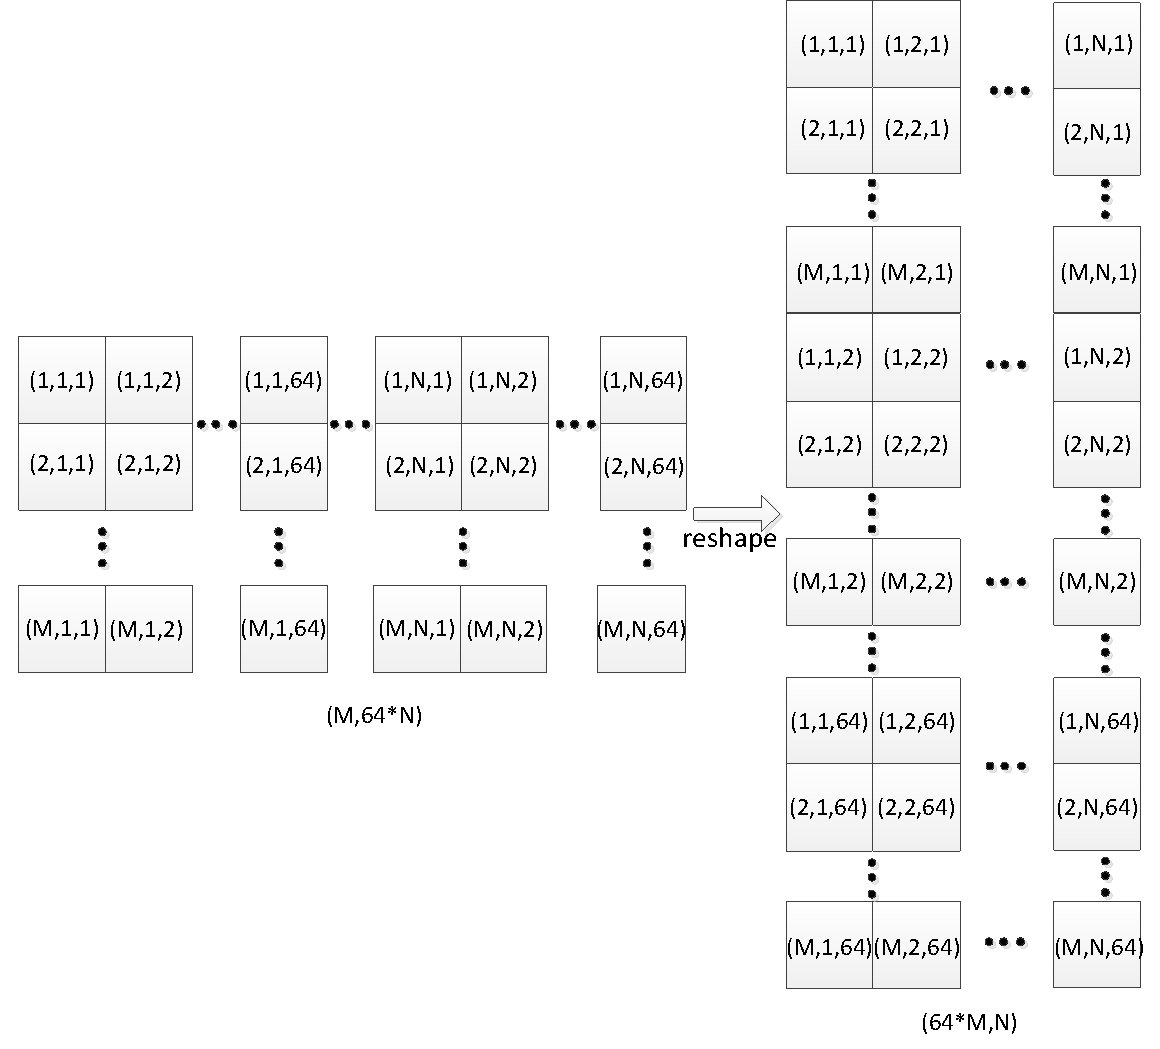
\includegraphics{figs/reshape.pdf}
}
\caption{For an input matrix, its size is $(M,N*\alpha *\alpha *\alpha)$, $\alpha$ is the tile size, here equal to 4. After the reshape kernel is applied, lots of small sub matrices with new layouts are generated}
\label{reshape}
\end{figure}

矩阵乘阶段的实现就相对简单了,这里直接通过调用cuBlas实现的,但需要进行$\alpha \times \alpha \times \alpha$次矩阵乘运算,每次矩阵乘的两个矩阵规模分别是$K \times C$与$C \times P$,得到$\alpha \times \alpha \times \alpha$个规模为$K \times P$的矩阵。这些结果矩阵也需要进行一次重排,通过$ReshapeOutput$这个kernel实现的,该kernel是从$\alpha \times \alpha \times \alpha$个矩阵的相同存储位置的元素一次组合在一起,产生$K \times P$个小块,每个小块的大小为$\alpha \times \alpha \times \alpha$。最后是对重排之后的$K \times P$个小块进行3D Winograd变换,与前两个变换类似,这里在用GPU实现时,每个线程块的线程数设为32,则线程块的配置为$(\frac{N}{32},\frac{D}{m},\frac{H}{m},\frac{W}{m},K)$。

\subsection{3D WMFA 算法的优化}
在\ref{baselineIm}中介绍的是在GPU平台上的一个baseline实现,在本小节中,将介绍针对GPU的两个优化方法,第一种优化方法是对齐访存,对齐访存可以使存储的访问更加高效,并且提高cache的命中率;第二种方法将变换与重排两步操作合并以减少全局存储的访问。

在GPU平台中,数据的存储顺序以及线程访问数据的方式将会影响GPU性能的发挥。在baseine实现中,输入图片数据是按照$NCDHW$的顺序存储的,即首先存储各个通道然后存储bach中的每一个输入,而由于线程块中的线程是在N所在维度方向进行划分的,这意味着处于同一个线程块中的线程访问的是处于batch中的不同输入图片,然而处于不同图片相同位置的数据在存储位置上是相隔很远的,GPU上的cache大小也是有限的,如同处于同一个线程块的线程所访问的数据相隔距离大于GPU的cache大小,则每个线程将独立地访问全局存储,这将导致大量的存储访问。因此,在第一种优化方法中,输入图片的存储顺序变成了$CDHWN$ ,这样输入数据最先存储的是N维中的数据,线程块中的32个线程访问的数据变成了连续存储,从全局存储中每次访存的数据都可以被使用,因此全局存储的访存带宽得到充分利用。同理,卷积核的存储顺序由$KTRSC$变为$CTRSK$,其中T、R、S为卷积核的大小,输出结果的存储顺序由$NDHWK$变为$KDHWN$。

在第一个优化方法的基础上,再采用第二优化方法,即将变换与重排两步操作合并。第二个优化方法的实质是减少对全局存储的访问,因为在基本实现的方法中,卷积核以及输入图片变换之后的结果是存储在全局存储中,然后进入下一个kernel执行重排操作,从全局存储中读出数据进行重排后写回全局存储器中。可以发现3D WMFA的基本实现中,重排使用单独的一个kernel来实现导致了大量的全局存储的访问,因此,很自然的想法就是将重排的实现合并到变换的kernel中,即在变换执行结束时,变换之后的结果在向全局存储存储时,直接存储到重排之后的正确位置中,紧接着就能进行矩阵乘运算。类似地,对矩阵乘的结果进行反变换之前,也可以不需要进行重排,变换时,直接从全局存储中读取相应的正确数据进行反变换。

由于全局存储器离计算单元相对最远,全局存储的访问对性能的影响非常大,第二个优化方法能够有效的减少对全局存储的访问。在\ref{experiment}节中,也将看到第二个优化方法对性能的影响。


\section{实验评测与分析}
\label{experiment}
\subsection{实验设置}
所有的实验都是在Geforce GTX 1080 GPU上测试的,该GPU计算性能强大,拥有20个多处理器,2560个CUDA 核心,8GB的显存大小,具体参数参考表\ref{my-label}。实验中软件环境主要是CUDA 8.0以及cublas和cuDNN库。
\begin{table}[]
\centering
\caption{Properties of the GeForce GTX 1080}
\label{my-label}
\begin{tabular}{l|l}
\hline
parameters                                    & values \\ \hline
CUDA capability major/minor version number    & 6.1    \\ \hline
Total amount of global memory                 & 8GB    \\ \hline
CUDA Cores                                    & 2560   \\ \hline
L2 Cache Size                                 & 2MB    \\ \hline
Warp size                                     & 32     \\ \hline
Total number of registers available per block & 64KB   \\ \hline
\end{tabular}
\end{table}


\subsection{3D WMFA 算法各优化方法的性能}
本实验测试了3D WMFA算法的各种实现在一个经典的3D卷积神经网络中的性能。这个经典的3D卷积网络是用来对视频进行分类的,该网络结构包含五层卷积层,表\ref{conv3d-info}列出了各个3D卷积层的参数以及包含的计算量。
\begin{table}[]
\centering
\caption{Convolution layers of a 3D network; the filter size in all layers is $3\times 3\times 3$, and the GFLOPS columns calculate the number of flops operations in each convolutional layer. Assume the batch size is $32$.}
\label{conv3d-info}
\begin{tabular}{|c|c|c|c|}
\hline
Layer & CxDxHxWxN       & K   & GFLOPS \\ \hline
conv1 & 3x16x112x112x32 & 32  & 16.65   \\ \hline
conv2 & 32x16x56x56x32  & 64  & 88.8  \\ \hline
conv3 & 64x8x28x28x32   & 256 & 88.8  \\ \hline
conv4 & 256x4x14x14x32  & 256 & 44.4   \\ \hline
conv5 & 256x2x7x7x32    & 256 & 5.55   \\ \hline
\end{tabular}
\end{table} 

由于第一层3D卷积层的通道数只有3,3D WMFA算法的实现代码暂不支持,因此,实验只对其它四层卷积层的3D WMFA实现进行了测试,比较了3D WMFA的基本实现以及两种优化的实现方法的性能。图\ref{result1}为3D WMFA算法的两种优化实现的性能相对于该算法的基本实现的性能加速。从结果中可以看到,各个卷积层的3D WMFA算法的实现中,第一种优化方法相对于基本实现取得了3 $\thicksim$ 4倍的加速。然而,第二种优化方法的实现相对于基本实现取得的最大加速比可以达到约42倍,最少也能达到约13倍的加速比。第一种优化方法使得存储访问变得更加高效,带宽得到了充分利用,对性能影响也是很显著的,而第二种优化方法能够减少大量不必要的全局存储访问,而全局存储访问的延迟在GPU的所有存储层次中是最大的,因此,第二种优化方法取得了非常好的优化性能。

\begin{figure}[tbh]%\small
\centering
\resizebox{0.8\textwidth}{!}{
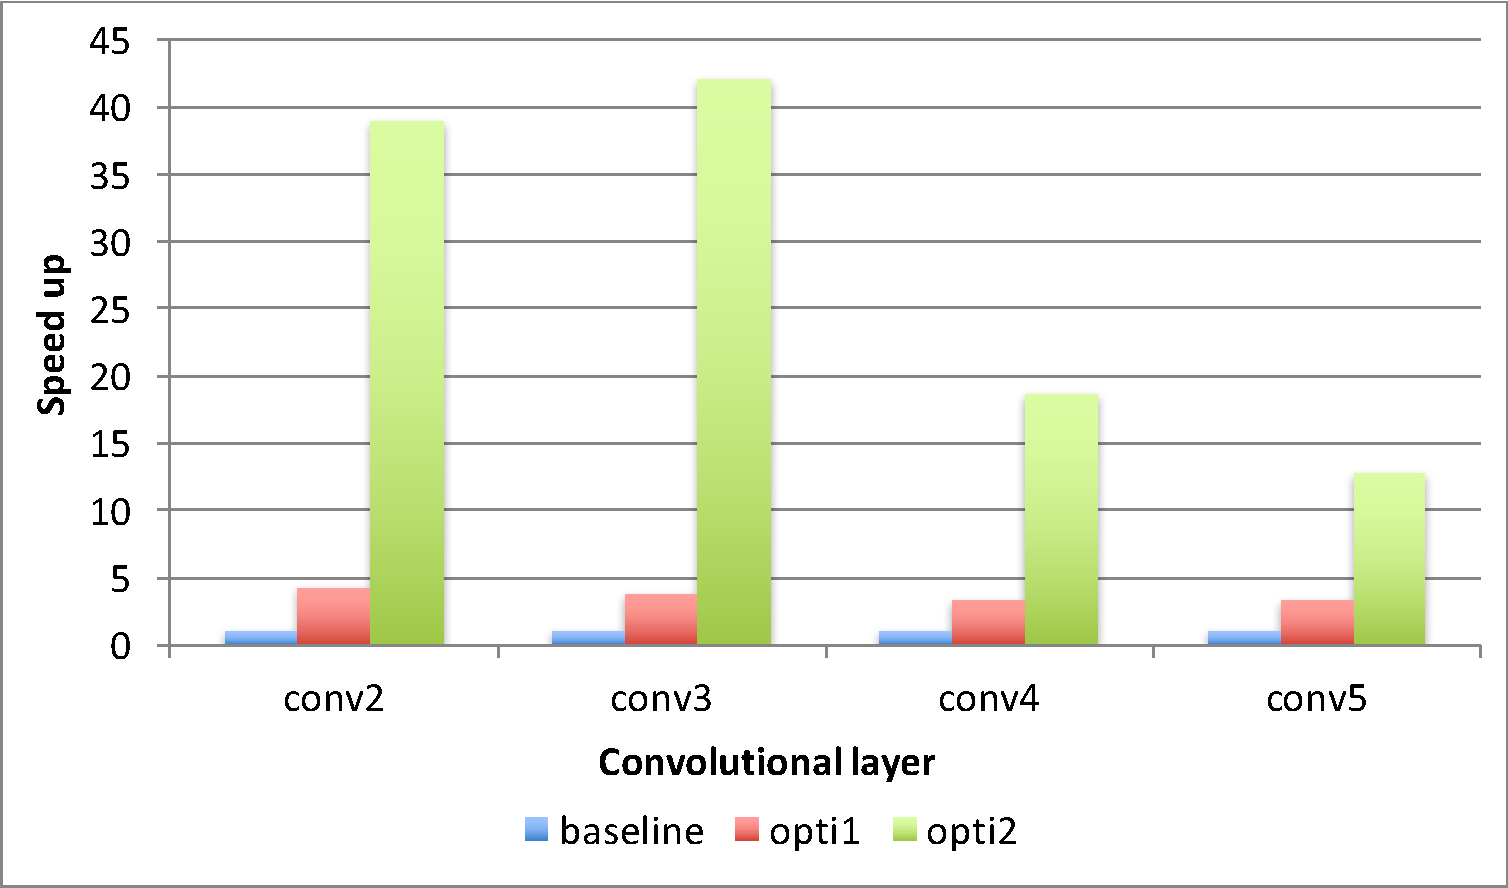
\includegraphics{figs/result1.pdf}
}
\caption{Speed up with different optimizations on 3D convolution layers}
\label{result1}
\end{figure}

\subsection{3D WMFA 算法各kernel执行时间分布}
第二个实验更好地研究了各个优化方法对各个kernel性能的具体影响。卷积层$conv3$的计算量算是最大的,因此第二个实验测试了3D WMFA算法的实现中的各个kernel在该层的性能变化。图\ref{result2}是3D WMFA算法的各个kernel在三种实现中的执行时间比较。无论是3D WMFA算法的基本实现方法还是第一个优化方法实现中,$ReshapeOutput$这个kernel在所有kernel中占用时间最长,这是因为该kernel中包含的全局访存次数是最多的。然而在第二个优化方法的实现中,由于重排部分已经被优化了,第二个优化方法的实现中所占时间最长的变为矩阵乘部分了,占了约$60\%$的时间。卷积核变换在这三种实现中所占比例都很低,这可以从计算复杂性分析部分找到理论上的支持。

\begin{figure}[tbh]%\small
\centering
\resizebox{0.8\textwidth}{!}{
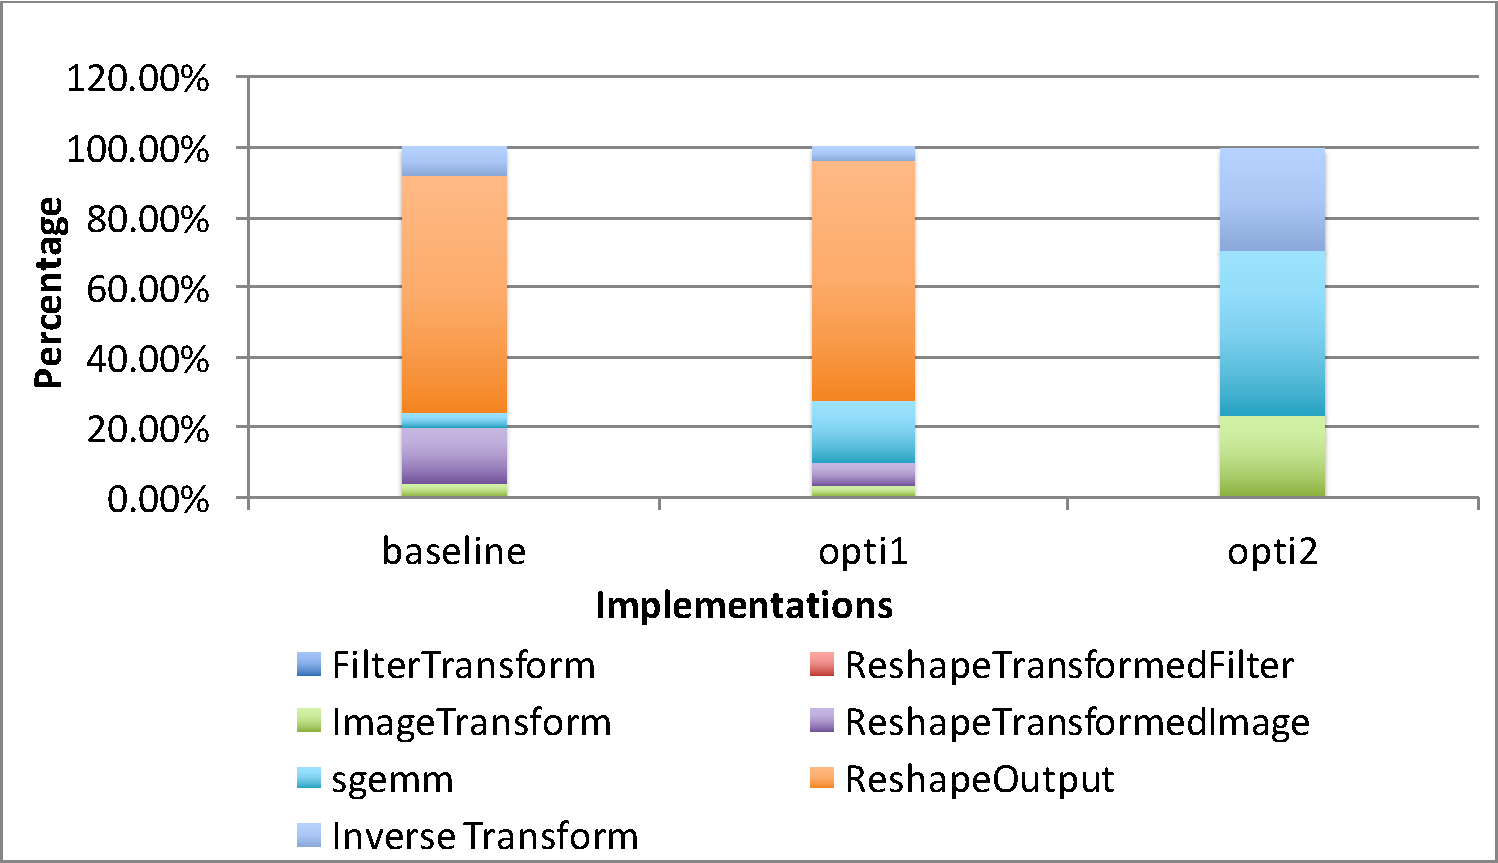
\includegraphics{figs/result2.pdf}
}
\caption{Time percentage distribution of each kernel in each implementation version for a specific convolution layer}
\label{result2}
\end{figure}

\subsection{3D WMFA 算法与其它卷级算法性能比较}
最后将3D WMFA算法的最优实现与当前GPU上的深度学习库进行性能比较,目前针对Nvidia 的GPU的深度学习库主要是cuDNN。cuDNN在对3D卷积计算的实现中,有两个可用的算法实现,一个是将卷积转化为矩阵乘,另一个是利用FFT 分块方法实现卷积。可以用$cuDNN$ $SGEMM$ 和 $cuDNN$ $FFT$ $Tiling$代表这两种方法,并用$3D WMFA$代表本章介绍的算法。图\ref{result3}为这三种卷积实现方法在四个卷积层的执行时间比较,对于$conv2$卷积层,$3D$ $WMFA$方法比$cuDNN$ $FFT$ $Tiling$方法慢$30$\%,然而比$cuDNN$ $SGEMM$方法性能要高,$cuDNN$ $FFT$ $Tiling$方法能够取得较快的速度是以消耗大量存储为代价的。由于参数$C$和$K$在卷积层$conv2$中比较小,导致在$3D$ $WMFA$方法中的矩阵乘规模比较小,影响了GPU性能的发挥。然而随着$C$和$K$两个参数的增大,我们看到对卷积层$conv3$、$conv4$以及$conv5$,$3D$ $WMFA$方法取得了比另两个方法更好的性能。如果将各个卷积层的执行时间累加起来得到总的执行时间,$cuDNN$ $SGEMM$方法的执行总时间为$132.6$ ms,$cuDNN$ $FFT$ $Tiling$方法的执行总时间为$135.4$ ms,而$3D$ $WMFA$方法的执行总时间为$108.2$ ms,比其它两种方法性能都要好。

\begin{figure}[tbh]%\small
\centering
\resizebox{0.8\textwidth}{!}{
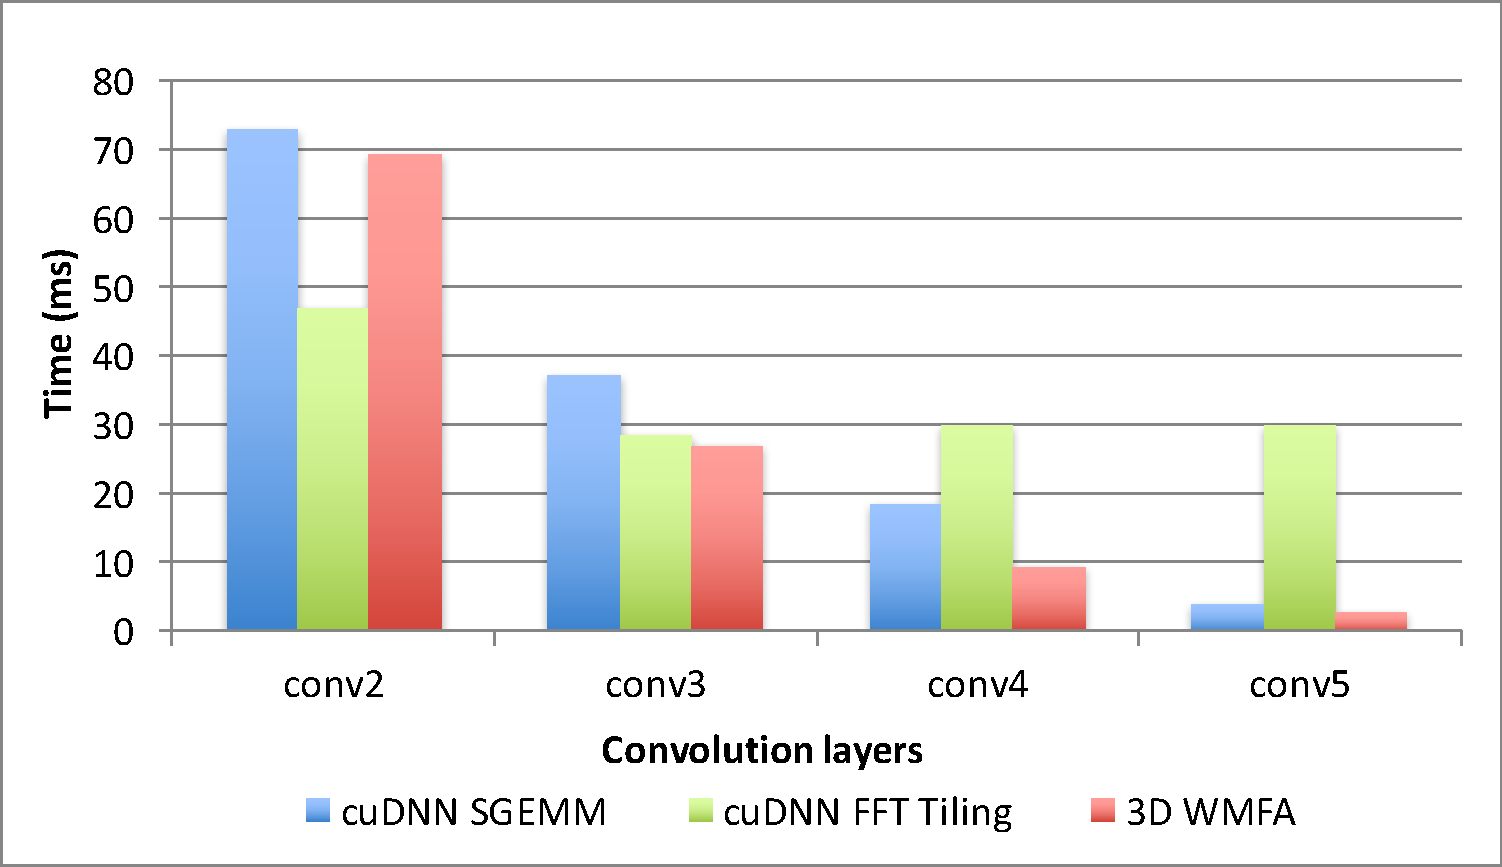
\includegraphics{figs/result3.pdf}
}
\caption{Execution time of different methods on 3D convolution layers}
\label{result3}
\end{figure}


可以进一步计算出$cuDNN$ $SGEMM$方法和$3D$ $WMFA$方法的浮点性能,表\ref{FlopsInfo}为这两种方法在各个卷积层的浮点计算性能。与$cuDNN$ $SGEMM$方法相比,$3D$ $WMFA$方法最高能达到$1.96$倍的加速,$3D$ $WMFA$方法取得最好的性能为4.72 TFLOPS,而GTX 1080的峰值性能为8.2TFLOPS,因此$3D$ $WMFA$方法能够达到峰值性能的$57.5$\%。

\begin{table}[]
\centering
\caption{Performance of cuDNN SGEMM versus that of the 3D WMFA on 3D convolution layers. Performance is measured in effective TFLOPS.}
\label{FlopsInfo}
\begin{tabular}{|c|c|c|c|c|c|}
\hline
\multirow{2}{*}{Layer} & \multirow{2}{*}{CxDxHxWxN} & \multirow{2}{*}{K} & \multicolumn{2}{c|}{TFLOPS} & \multirow{2}{*}{speedup} \\ \cline{4-5}
                       &                            &                    & cuDNN SGEMM       & 3D WMFA        &                          \\ \hline
conv2                  & 32x16x56x56x32             & 64                 & 1.21        & 1.28          & 1.05                     \\ \hline
conv3                  & 64x8x28x28x32              & 256                & 2.38        & 3.31          & 1.39                     \\ \hline
conv4                  & 256x4x14x14x32             & 256                & 2.4         & 4.72          & 1.96                     \\ \hline
conv5                  & 256x2x7x7x32               & 256                & 1.46        & 2.1           & 1.44                     \\ \hline
\end{tabular}
\end{table}

\section{小结}
2D卷积神经网络的成功应用,使得3D卷积神经网络的研究逐渐盛行,而3D卷积神经网络主要需要解决的问题就是计算量大的问题。传统的卷积计算方法比如矩阵乘和FFT变换方法并不能有效地应用到3D卷积计算中,本章采用的3D WMFA算法,可以从理论上证明这个方法能够有效地减少3D卷积的计算量并且不会增加额外的存储开销。

本章从1D和2D WMFA算法的推导开始,进而推导出了3D WMFA算法的形式,并对该算法的计算复杂行进行了理论分析,理论上,该算法能将核心计算降低到原来计算的$30$\%,代价是增加一些额外的变换开销,但这些变换开销与核心的浮点计算相比,占的比例比较小。

在3D WMFA算法的具体实现中,本章主要介绍了GPU平台下,对算法中变换进行了高效地实现。虽然算法中涉及的几个变换的计算量不大,但由于变换中涉及到对全局存储的访问,因此,本章介绍了对存储访问的两种优化方法,一种是对齐访存,使得访存更加高效,存储带宽得到充分利用,另一种是减少大量不必要的全局存储访问,显著地减少访存时间,这两种优化方法都取得了很好的效果。

本章最后对3D WMFA的优化实现与cuDNN中对3D卷积的两种实现方法进行了比较,在某些卷积层3D WMFA算法达到了近2倍的加速,取得了近60\%的峰值性能。

3D WMFA算法有多种形式,本章介绍的只是其中一种形式,就是在变换中,变换的结果小块大小为2,变换得到的结果小块可以是其它值,该值越大,卷积计算中的浮点运算量将减小得越多,但是变换开销将增大,因此,对于变换结果的小块大小的选取应该会有一个最优值,使得最后3D WMFA算法的整体计算复杂性最低。这个工作可以作为本课题未来的研究工作。
























